\chapter{Results}

Usability tests make it possible to verify if the design meets the expectations of the target group and offer a way to discover unexpected problems that are hard to track by the developers themselves. Test persons have a fresh look on the application and can provide useful insights in the way they interpret visual elements of the user interface.\\

In addition, the technical evaluation considers the effect of the implementation, ensuring that the user is not hindered by performance issues or similar problems.


\section{Usability test}

The graphical user interface is designed for use by physical therapists. As such, acquiring feedback from therapists is essential in developing an interface that is both useful and easy to use. The process of the usability test is described, followed by an overview of the most important results of the evaluation itself and an interpretation of these results.


\subsection{Description of the test}

A usability test is conducted with physical therapist Dries Lamberts at Windekind Leuven, an organization that focuses on the education of children with disabilities and offers a full program to assist them with their specific difficulties. For this test, the Kinect camera is connected to a computer that runs the application and, positioned on a desk at hip height. The user indicates that he is familiar with using the Kinect camera and motion-based games.\\

A short introduction on the purpose of the application is given to the test person for reference. After that, he is presented with several tasks and is asked to apply the think-aloud protocol in order to obtain as much information as possible about the interaction with the application and the thoughts of the user while doing so.\\

In preparation of the usability test, gestures are pre-recorded that both serve the purpose of testing the robustness of the application as well as having a fallback plan in case problems arise during the test.\\

One task is to watch the pre-recorded gestures and control a game called Space Invaders using the pre-recorded gestures. This is a game that has an avatar move left or right on the screen and shoot bullets (see figure \ref{fig: space_invaders}). As such, four gestures are pre-recorded: one gesture that allows the avatar to move to the left, one to move to the right, one to shoot bullets and a neutral gesture that is linked to no keyboard key. At this point, it is explained to the user that a neutral gesture is required in order to have a gesture to which no keys are linked. This is explained without going into detail about the specifics of SVM. The goal of this task is twofold. Firstly, the task is used to verify if the test person is able to watch replays of the pre-recorded gestures without any guidance and to learn what gestures are pre-recorded without additional information. After this is done, it is explained to the user how the gestures and keyboard keys are linked together. Secondly, it makes it possible to confirm if a correct prediction of a gesture execution does not depend on the person performing the gesture, as problems can arise due to the person recording the gestures and the person playing a game having a very different physique.\\

\begin{figure}[H]
\begin{center}
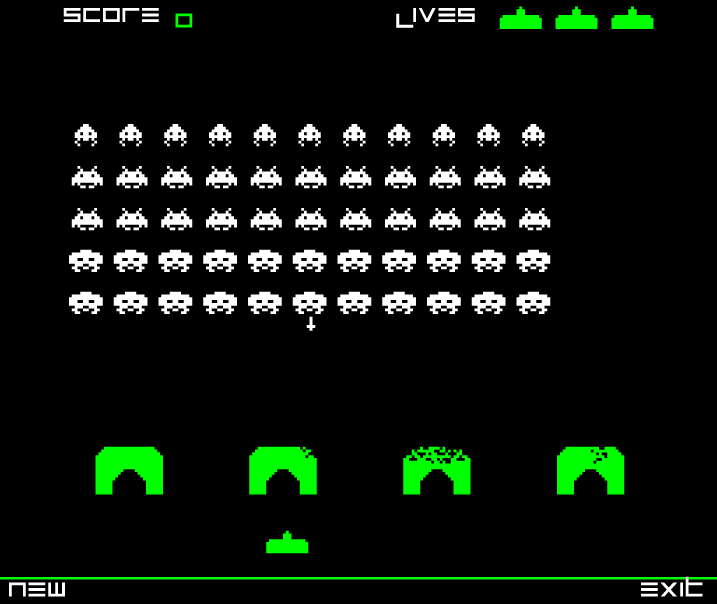
\includegraphics[width=8cm]{SpaceInvaders.png}
\caption{\emph{Screenshot from Space Invaders}}
\label{fig: space_invaders}
\end{center}
\end{figure}

Another task is to play the game Sokoban Geek. This puts the gamer in control of an on-screen avatar that can move up, down, left or right. Walking into boulders allows the player to move them in order to solve a puzzle (see figure \ref{fig: sokoban_geek}). The game is shown to the test person and after trying the game, he decides how many gestures are required to play the game. Then, he comes up with different gestures for each input and records three trainings for each of them. The test person is asked to delete a recorded gesture and record it again. After recording all gestures, he tries to play the game. The goal of this task is to check how the test person reacts to the recording elements of the interface and if it is clear how to interact with them without assistance.\\

\begin{figure}[H]
\begin{center}
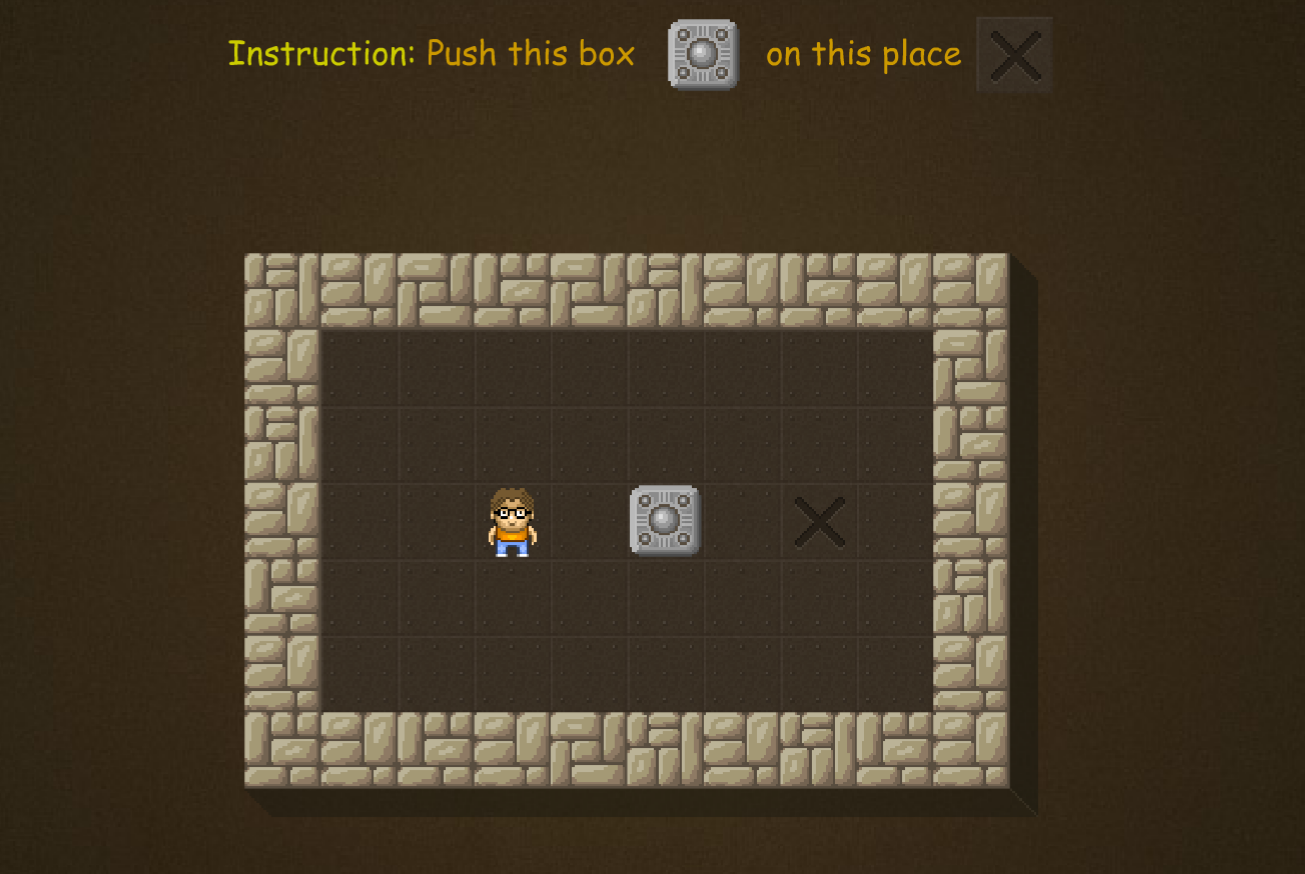
\includegraphics[width=8cm]{SokobanGeek.png}
\caption{\emph{Screenshot from Sokoban Geek}}
\label{fig: sokoban_geek}
\end{center}
\end{figure}

\newpage

With permission of the test person, during the entire test, the computer screen is recorded, as well as everything said, for analysis purposes. The system usability score (SUS) allows to obtain a numeral indication of the usability of the application based on ten questions. At the end of the usability test, the user is asked to fill out a questionnaire with these ten questions. While this score gives an indication of the application's usability, it is not possible to draw firm conclusions as a larger number of test persons is required in order for the usability score to be statistically relevant.


\subsection{Results}

This section will describe how the physical therapist interacted with the UI that was seen in chapter \ref{interface description}, there all the figures to which this section refers are shown.

For the first task, the user notices the recorded gestures in a list on the right-hand side of the screen. By trying to move its avatar's hand to align with the previews of the recordings, he notices that it is possible to scroll through the list of recordings. He also notices the delete option next to the recordings list and indicates that he is anxious about deleting one of the recorded gestures because of the rather aggressive red color of the progress bar.\\

Watching a replay of the recorded gestures initially is not clear to the user. He tries to drag one of the gestures to the square on the left hand-side of the screen, which is intended to be the display screen. He notices that this is not possible, but makes several attempts do this. After that, he indicates that he can't find it and looks at the interface without trying to interact with anything. To replay a recorded gesture, the user can point with the avatar's hand to the recorded gesture in the orange area of the scrollbar, previously referred to as the selection box area. At that point, a replay of that gesture is displayed automatically. The replay stops while scrolling through the list or when not pointing at the gesture in the selection box area. The user did this several times during this task subconsciously, without noticing that a replay started playing at the left side of the screen. A factor adding to this problem is the fact that the recordings were displaying a posture rather than a gesture, which in fact is a static image instead of an animation. The user required assistance to complete this task. He was able to do this after knowing that the gesture in the selection box area is displayed at the left-hand side square.\\

After watching replays of the recorded gestures, the user is able to replicate in real life what gestures are recorded and displayed on-screen. When the Space Invaders game is started, the user has no problem interacting with the game and does not require any assistance. He is able to control the in-game avatar subtly and meet the game objectives. After asking for his experience with the controls, he indicates that the controls are responsive and that he does not experience any lag.\\

For the second task, the user gets the chance to see what the Sokoban Geek game looks like and how it is played. After that, he states that he needs five gestures to play the game. Four gestures are linked to a directional keyboard key and one gesture that serves as the neutral gesture. To record a gesture, it is required that the user hovers the hand of the on-screen avatar over the grip of the pulling cord, makes a fist, and move his fist down to start recording. This translates to pulling the displayed cord. When trying to start recording the first gesture, the user pulls the cord without any problems. The recording screen appears and he starts performing a gesture when the interface indicates that recording has started. He stands still when he is done with the gesture and the recording stops automatically.\\

Upon being asked to delete the gesture he just recorded, he needs no assistance to push the gesture object to the right into a box indicating that the gesture can be deleted. He indicates that his earlier anxiousness of deleting a gesture by accident is unnecessary, as it requires some effort to perform this deleting action and it is hard to do it by accident.\\

\newpage

When trying to record a gesture the second time, the user is unaware that he is required to close his hand into a fist to pull the cord. He tries hovering over the grip and moving his hand down and indicates that he isn't sure why recording does not start this time. Only after several tries, he tries closing his hand to pull the cord, activating the recording screen. He states that he did not know that closing the hand was required and that he did that by accident to record the first gesture. He indicates that he has experience using the Kinect camera for other games and that these games never required to close a hand, so he was unaware that the Kinect is able to make a distinction between open and closed hand.\\

The user notices clearly that the recording of a gesture stops when he stands still. Because he was not aware of this, one gesture was not recorded the intended way, but the user was able to delete this gesture and record a new one without assistance. The user also noticed that the light blue and dark blue puppets behind his puppet during the recording screen indicate the beginning and ending position of his first gesture. He states that this feature is very useful for repeating the original gesture.\\

When trying to watch a replay of a recorded gesture, he is not sure if he needs to point at the gesture with open or closed hand. Although both cases function in the same way, the user states that using a closed hand feels like the application responds better. He also wondered whether the recording would distinguish the difference between open and closed hand, but concludes that it does not because the replay of the recording does not show any difference. This is as intended. While watching the replay, he noted that it is not possible to accurately tell what a gesture looks like when stretching for instance an arm straight ahead. The replay does not provide any information about depth.\\

After the user records all gestures, he is able to play the game. However, the gesture that is linked to the left arrow key does not respond. The user is asking if the key is linked correctly to the gesture and thinks this is the problem. He misses feedback about what gesture is linked to what key, though it should be noted that the concept is that keys would be assigned on a different screen in a full application. After verifying for the user that the key is linked correctly, we present him with the question of how he would handle this problem without any assistance. He suggested to delete the recorded gestures and record them again. After doing this, the user is able to play the game without further problems. Analogous to the situation of playing the first game, the user plays the second game with similar ease.\\

The entire user test approximately took 45 minutes. After the test, the user asked because of his own experience with disabled children if very small gestures are supported by the application and if the application can be used for other purposes than playing games. An example he thought of was using gestures to type words using sign language. He also added that he was glad that use of the space bar is supported by the application, as he has experience with similar projects that do not support the space bar, while it is one of the most used keys in computer games. However, a lot of games the children are interested in require the ability to point with a cursor on-screen. This is a feature he would appreciate. Finally, he stated that he is very interested in using the application, allowing disabled children to play games and exercise while doing so.


\subsection{Discussion}

The physical therapist proved to understand the concept of the application. This shows that it is possible for persons without programming knowledge to use the application for recording gestures and controlling computer games. He also understands that the use of the application is not limited to games and can also be used for other computer applications that require keyboard input.\\

A few tries are required to get familiar with how to start recording and how to end it. In particular, without prior knowledge or experience, more feedforward is required to communicate that the hand needs to be closed when pulling the cord and that the user needs to stand still to stop recording. However, after a few tries, it is possible to record multiple gestures in succession without any of them not being recorded as intended.\\

Replaying recorded gestures requires the user to align his on-screen hand with the gesture inside the selection box area of the scrollbar. There is no form of feedforward indicating that performing this action results in the gesture being replayed. The feature is intended for the user to be discovered while scrolling through the gestures or while trying to delete a gesture. As such, this can be confusing to the user.\\

Both the actions of recording gestures and replaying recorded gestures are performed faster after having experienced this firsthand. The provided feedforward is too subtle to immediately make it clear what actions are expected. To improve this, it is either possible to provide more explicit feedforward, or to introduce the user to the most important functions using a tutorial.\\

When playing the games using gestures, the test person appears to be very engaged in them and the way they are controlled. This is an indication that not only the application succeeds in its purpose of playing a game with gesture-based input, it also can make for a pleasant experience.


\section{Technical evaluation}

The application is developed with the Microsoft Visual Studio integrated development environment (IDE) in C$++$ and can run on Windows operating systems. This limitation is due to the use of the IDE's visual interface editor and Direct2D, as well as the feature of saving and loading data files. The application is tested to run on both Windows 8.1 and Windows 10 machines.\\

All of the required files for running the application, including resource images, take up approximately 20 MB of space. Saving all gestures needed for playing a game takes up approximately an additional 0.6 MB of space. This depends on the number of gestures recorded, the number of trainings done for each gesture and the duration of each gesture.\\

The application refreshes the interface at a rate of 30 frames per second (FPS), which is limited by the output of the Kinect camera. The Kinect also introduces limitations related to the environment and the user. These limitation are that overly lit rooms make it harder for the camera to track a person. The same is true for persons wearing black or reflecting clothing. These findings are in accordance to Microsoft's guidelines for using the Kinect \cite{MicrosoftGuidelines}.